\documentclass[12pt, twoside]{article}
\usepackage[letterpaper, margin=1in, headsep=0.2in]{geometry}
\setlength{\headheight}{0.6in}
%\usepackage[english]{babel}
\usepackage[utf8]{inputenc}
\usepackage{microtype}
\usepackage{amsmath}
\usepackage{amssymb}
%\usepackage{amsfonts}
\usepackage{siunitx} %units in math. eg 20\milli\meter
\usepackage{yhmath} % for arcs, overparenth command
\usepackage{tikz} %graphics
\usetikzlibrary{quotes, angles}
\usepackage{graphicx} %consider setting \graphicspath{{images/}}
\usepackage{parskip} %no paragraph indent
\usepackage{enumitem}
\usepackage{multicol}
\usepackage{venndiagram}

\usepackage{fancyhdr}
\pagestyle{fancy}
\fancyhf{}
\renewcommand{\headrulewidth}{0pt} % disable the underline of the header
\raggedbottom
\hfuzz=2mm %suppresses overfull box warnings

\usepackage{hyperref}

\fancyhead[LE]{\thepage}
\fancyhead[RO]{\thepage \\ Name: \hspace{4cm} \,\\}
\fancyhead[LO]{BECA / Dr. Huson / Geometry\\*  Unit 8: Year-to-date Regents review\\* 10 March 2023}

\begin{document}

\subsubsection*{8.8 Unit exam: Regents standards \hfill v2}
\begin{enumerate}
\item What is the sum of the measures of two complementary angles? \hfill HSG.CO.C.10
\begin{multicols}{2}
\begin{enumerate}
  \item $45^\circ$
  \item $90^\circ$
  \item $120^\circ$
  \item $180^\circ$
\end{enumerate}
\end{multicols}

\item A regular octagon is rotated about its center. Which degree measure will carry the polygon onto itself? 
\begin{multicols}{2}
\begin{enumerate}
  \item $30^\circ$
  \item $45^\circ$
  \item $60^\circ$
  \item $72^\circ$
\end{enumerate}
\end{multicols}

\item Two parallel lines intersect a transversal. The same side interior angles measure m$\angle 1 = 2x+30$ and m$\angle 2 = x+75$. What is the value of $x$?
\begin{multicols}{2}
  \begin{enumerate}
    \item $25^\circ$
    \item $34^\circ$
    \item $45^\circ$
    \item $53^\circ$
  \end{enumerate}
  \begin{tikzpicture}[scale=1]
    \draw [<->, thick] (3,0)--(8.5,0);
    \draw [<->, thick] (2.5,2)--(8,2);
    \draw [<->, thick] (5,-1)--(3,3);
    \node at (5.3, 1.75){m$\angle 1 = 2x+30$};
    \node at (6.1, 0.25){m$\angle 2 = x+75$};
  \end{tikzpicture}
  \end{multicols}

\item Given $\triangle ABC$ with $\overrightarrow{ACD}$. \hfill HSG.CO.C.10
  \begin{center}
    \begin{tikzpicture}[scale=0.7]
    \draw [thick, <-]
    (10,0)node[below]{$D$}--
    (0,0)node[below]{$A$}--
    (4,4)node[above]{$B$}--
    (7,0)node[below]{$C$};
    \node at (0.9,0.4){1};
    \node at (6.2,0.4){3};
    \node at (7.2,0.4){4};
    \node at (4,3.3){2};
  \end{tikzpicture}
  \end{center}
  Which equation is always true?
  \begin{multicols}{2}
  \begin{enumerate}
    \item $m\angle 4 = m\angle 3 - m\angle 2$
    \item $m\angle 3 = m\angle 1 + m\angle 2$
    \item $m\angle 3 = m\angle 1 - m\angle 2$
    \item $m\angle 4 = m\angle 1 + m\angle 2$
  \end{enumerate}
  \end{multicols}

\newpage
\item What is the midpoint of $\overline{AB}$, with $A(1.7,-2)$ and $B(4.5,-5.2)$? \hfill GPE.B.6
\begin{multicols}{2}
  \begin{enumerate}
    \item $(0.3,-7.2)$
    \item $(3.6,-1.6)$
    \item $(7.2,-3.2)$
    \item $(3.1,-3.6)$
  \end{enumerate}
  \end{multicols} \vspace{1cm}

\item The endpoints of directed line segment $PQ$ have coordinates of $P(-7,-5)$ and $Q(5,3)$. What are the coordinates of point $A$, on $\overline{PQ}$, that divide $\overline{PQ}$ into a ratio of 1:3?
\begin{multicols}{2}
  \begin{enumerate}
    \item $(-1,-1)$
    \item $(-4,-6)$
    \item $(-4,-3)$
    \item $(-6,-4)$
  \end{enumerate}
  \end{multicols} \vspace{2cm}

\item In the line segment $\overline{ABC}$, $\overline{AB}$ is twice as long as $\overline{BC}$. $AB=12x-6$ and $AC=15x+9$. Find $BC$.
  \begin{multicols}{2}
  \begin{enumerate}
    \item $31$
    \item $33$
    \item $36$
    \item $42$
  \end{enumerate}
  \end{multicols} \vspace{1cm}

\item Lou has a solid clay brick in the shape of a rectangular prism with a length of 8 inches, a width of 3.5 inches, and a height of 2.25 inches. If the clay weighs 1.055 oz/in$^3$, how much does Lou's brick weigh, to the nearest ounce? 
  \begin{multicols}{2}
    \begin{enumerate}
    \item $53$
    \item $59$
    \item $66$
    \item $71$
  \end{enumerate}
  \end{multicols} \vspace{1.5cm}
  
\item The base of a pyramid is a rectangle with a width of 4.6 cm and a length of 9 cm. What is the height, in centimeters, of the pyramid if its volume is 82.8 cm$^3$? \hfill HSG.GMD.A.3
\begin{multicols}{2}
  \begin{enumerate}
    \item $6$
    \item $7$
    \item $8$
    \item $10$
  \end{enumerate}
  \end{multicols} \vspace{0.5cm}

\newpage
\item What is the slope of a line perpendicular to the line with the equation $y=-2x-15$?
  \begin{multicols}{2}
    \begin{enumerate}
      \item $-\frac{1}{2}$
      \item $\frac{1}{2}$ 
      \item $-2$
      \item $2$
    \end{enumerate}
  \end{multicols}

\item What is an equation of the line that passes through the point $(-3,7)$ and is perpendicular to a line with equation $y=\frac{2}{3}x+5$?
  \begin{multicols}{2}
    \begin{enumerate}
      \item $y-7=-\frac{3}{2}(x+3)$
      \item $y-7=\frac{3}{2}(x-3)$ 
      \item $y+7=\frac{3}{2}(x+3)$
      \item $y+7=-\frac{3}{2}(x-3)$
    \end{enumerate}
  \end{multicols}

\item What is an equation of the image of the line $y=\frac{3}{2}x-4$ after a translation down two?
\begin{multicols}{2}
  \begin{enumerate}
    \item $y=\frac{3}{2}x-2$
    \item $y=\frac{3}{2}x-6$
    \item $y=-\frac{2}{3}x-2$
    \item $y=-\frac{2}{3}x-6$
  \end{enumerate}
\end{multicols}

\item Which three-dimensional figure will result when a rectangle 6 inches long and 5 inches wide is continuously rotated about the longer side?
  \begin{enumerate}
    \item a rectangular prism with a length of 6 inches, width of 6 inches, and height of 5 inches
    \item a rectangular prism with a length of 6 inches, width of 5 inches, and height of 5 inches
    \item a cylinder with a radius of 5 inches and a height of 6 inches
    \item a cylinder with a radius of 6 inches and a height of 5 inches
  \end{enumerate}

\item The figure below shows a rhombus with noncongruent diagonals.
  \begin{center}
    \begin{tikzpicture}[scale=0.7]
      \coordinate (A) at (0, 0); %[label=above left:$P$]
      \coordinate (B) at (4, 0);
      \coordinate (C) at (5, 3.87);
      \coordinate (D) at (1, 3.87);
      \draw [thick] (A)--(B)--(C)--(D)--cycle;
      \draw [thick] (A)--(C);
      \draw [thick] (B)--(D);
      %\draw [thick, xshift=2cm, yshift=2.5cm] (85:3);
    \end{tikzpicture}
  \end{center}
  Which transformation would \emph{not} carry this rhombus onto itself?
    \begin{enumerate}
      \item a reflection over the shorter diagonal
      \item a reflection over the longer diagonal
      \item a clockwise rotation of $90^\circ$ about the intersection of the
      diagonals
      \item a counterclockwise rotation of $180^\circ$ about the intersection of the
      diagonals
    \end{enumerate}
  
\newpage
\item In the diagram below of right triangle $ABC$, $AC=4$, and $BC=2$. Find the length $AB$ using the Pythagorean theorem.
  \begin{multicols}{2}
    \begin{enumerate}
      \item $6$
      \item $2\sqrt{5}$ 
      \item $5\sqrt{2}$
      \item $\sqrt{12}$ 
    \end{enumerate}
      \begin{tikzpicture}[scale=0.7]
      \draw [thick]
        (0,0)node[below]{$A$}--
        (-6,4)node[above]{$B$}--
        (-6,0)node[below]{$C$}--cycle;
        \draw (-6,0)++(0.5,0)--++(0,0.5)--+(-0.5,0);
        \node at (-3,0)[below]{$4$};
        \node at (-6.5,2){$2$};
    \end{tikzpicture}
  \end{multicols}

\item What is the distance between the points $(1,11)$ and $(7,2)$ rounded to \emph{the nearest tenth}?
  \begin{multicols}{2}
    \begin{enumerate}
      \item $7.7$
      \item $8.1$ 
      \item $8.8$
      \item $10.8$
    \end{enumerate}
  \end{multicols} \vspace{1cm}

\item Rhombus $BECA$ has vertices $B(3,2)$4, $E(7,5)$, $C(11,2)$, and $A(7,5)$. What is the perimeter of rhombus $BECA$?
  \begin{multicols}{2}
    \begin{enumerate}
      \item $16$
      \item $18$ 
      \item $20$
      \item $24$
    \end{enumerate}
  \end{multicols}

\item Which point is further from the origin, $(-13,0)$ or $(5,-12)$?
  \begin{multicols}{2}
    \begin{enumerate}
      \item $(-13,0)$
      \item $(5,-12)$ 
      \item both are equidistant from the origin
      \item one or more distance is undefined
    \end{enumerate}
  \end{multicols}

\item What equation represents a line with a $y$-intercept of $b=-5$ that is parallel to the line represented by $y=\frac{2}{5}x+1$?
  \begin{multicols}{2}
    \begin{enumerate}
      \item $y=\frac{5}{2}x-5$
      \item $y=\frac{5}{2}x+5$
      \item $y=\frac{2}{5}x-5$
      \item $y=\frac{2}{5}x+5$
    \end{enumerate}
  \end{multicols}

\item Determine and state an equation of the line perpendicular to the line\\ $2x-y=7$ and passing through the point $(3,11)$.
  \begin{multicols}{2}
    \begin{enumerate}
      \item $y-11=-\frac{1}{2}(x-3)$
      \item $y-11=\frac{1}{2}(x-3)$ 
      \item $y+11=2(x-3)$
      \item $y+11=-2(x-3)$
    \end{enumerate}
  \end{multicols}


\end{enumerate}
\end{document}